\documentclass[10pt,a4paper]{article}
\usepackage{geometry}
\usepackage[utf8]{inputenc}
\usepackage{CJKutf8}
\usepackage{graphicx}
\usepackage{epsfig}
\usepackage{mathptmx}
\usepackage{times}
\usepackage{amsmath}
\usepackage{amssymb}
\usepackage{cite}
\usepackage{subfigure}
\usepackage{subfig}
\usepackage{verbatim}
\usepackage{multirow}
\usepackage{bm}
\usepackage{float}
\usepackage{etoolbox,xstring,mfirstuc,textcase}
\usepackage{indentfirst}
\usepackage{enumerate}
\author{沈艳晴}
\title{Assignment1--相机参数标定}
\geometry{left=3.18cm, right=3.18cm, top=2.54cm, bottom=2.54cm}

\begin{document}
\begin{CJK*}{UTF8}{gbsn}
\CJKindent%中文缩进专用
\maketitle


\begin{abstract}
经典的小孔成像模型,是通过将三维空间中的点投影到成像平面,得到了图像。
图像与三维空间的点存在一一对应的关系,求解这种对应关系的本质是求解相机的内、外参数。
通过使用具有某些先验信息的标定物,对相机的内、外参数进行求解同时求解畸变参数,为之后的图像处理与三维空间建立联系提供数学基础,并对镜头畸变进行校正。
本文通过使用张氏标定法对采集的图像进行处理,求解对应相机的参数。
\end{abstract}

\section{针孔成像模型}

在对图像与3D空间对应关系的研究中,常用的理想模型为摄像机针孔模型(Pinhole Camera Model)。
示意图如Fig. \ref{fig:camera1}.
\begin{figure}[htbp]
    \centering
    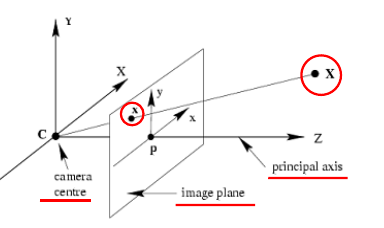
\includegraphics[height=4.5cm,width=8.5cm]{/home/midou/class/cv/cv_1report/1.png}
    \caption{小孔成像简化示意图}
    \label{fig:camera1}
\end{figure}

将三维物体成像过程抽象为Fig. \ref{fig:camera2}中的数学模型,为点的匹配建立数学上的对应关系。
\begin{figure}[htbp]
    \centering
    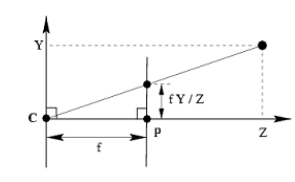
\includegraphics[height=4.5cm,width=8.5cm]{/home/midou/class/cv/cv_1report/2.png}
    \caption{小孔成像数学模型}
    \label{fig:camera2}
\end{figure}

\section{相机坐标系统}
\subsection{坐标系概述}
相机标定问题中一共涉及到四个坐标系统,分别是世界坐标系($X_w,Y_w,Z_w$)、相机坐标系($X_c,Y_c,Z_c$)、图像物理坐标系(x,y)、像素坐标系(u,v);

\begin{itemize}
    \item 世界坐标系与摄像机和成像平面本身独立,我们将根据世界坐标系对摄像机姿态进行描述。在实际工程中,可根据具体情况自由选择。
    \item 相机坐标系的原点位于镜头光心处,z轴为为光轴,垂直于成像平面;x、y轴则分别平行于相平面的两边。
    \item 图像物理坐标系的原点是光轴与成像平面的交点,即主点,也就是图像中心点。x、y轴与相机坐标系一致。
    \item 图像像素坐标系是对物理坐标系进行了尺度变换和原点平移。一般情况下,将图像左上角定义为原点,单位从毫米转换为像素。 
\end{itemize}

其中世界坐标系和相机坐标系为3维坐标系统,图像物理坐标系和像素坐标系为成像平面上的2维坐标系统。

他们之间存在一定的转换关系,为三维空间点与图片像素点建立对应关系。
\subsection{世界坐标系到相机坐标系}
两者之间的转换为刚体变换,描述的是相机本身相对于参考系的姿态,即\textbf{外参矩阵}。

表示如下:
\[Matrix_{Ex} = \begin{bmatrix}
R & T \\
0^{T} & 1
\end{bmatrix}\]
某三维点在相机系下坐标表示为$X_{cam}$,世界系表示为$X_{w}$,使用齐次坐标表示转换关系如下:
\begin{equation}
\label{ex}
X_{cam} = \begin{bmatrix} X_c \\ Y_c \\ Z_c\end{bmatrix}
= Matrix_{Ex} \cdot X_w= Matrix_{Ex} \cdot\begin{bmatrix}X_w \\ Y_w \\ Z_w\end{bmatrix}
\end{equation}

\subsection{相机坐标系到图像物理坐标系}
表现的是投影的过程。

如Fig. \ref{fig:camera2},根据三角形相似原理,相机系下3维点的坐标$(X,Y,Z)$经过直线投影,
对应的2维像平面坐标为$(f\frac{X_c}{Z_c}, f\frac{Y_c}{Z_c}$,其中$f$表示相机的焦距。
同样的,为了用简单的矩阵乘法表示转换过程,我们引入齐次坐标,表达如下:
\begin{equation}
\label{eq:in1}
\begin{bmatrix}
fX \\ fY \\ Z
\end{bmatrix} = 
\begin{bmatrix}
f &   &   & 0 \\
  & f &   & 0 \\
  &   & 1 & 0
\end{bmatrix} \begin{bmatrix} X \\ Y \\ Z \\ 1 \end{bmatrix}
=
\begin{bmatrix}
f &   &   \\
  & f &   \\
  &   & 1
\end{bmatrix} \begin{bmatrix}  I & | & \mathbf{0}\end{bmatrix} \begin{bmatrix} X \\ Y \\ Z \\ 1 \end{bmatrix}
\end{equation}

\subsection{图像物理坐标系到像素坐标系}
该过程实现了坐标单位和坐标系原点的平移变换。将距离单位的坐标转换为像素单位的坐标,并将坐标系原点从图像正中心移动到图片的左上角。$m_x, m_y$表示每米的像素数。使用齐次坐标表示变化过程:
\begin{equation}
\begin{bmatrix}
u \\ v \\ 1
\end{bmatrix}=
\begin{bmatrix}
m_x & 0 & u_0 \\
0 & m_y & v_0 \\
0 & 0 & 1
\end{bmatrix} \begin{bmatrix} x \\ y \\ 1 \end{bmatrix}
\label{eq:in2}
\end{equation}

\subsection{标定矩阵}
标定矩阵$P$包括两部分,\textbf{外参矩阵}和\textbf{内参矩阵}。
其中外参矩阵如公式(\ref{ex})所示,内参矩阵$K$包括公式(\ref{eq:in1})和(\ref{eq:in2}).
\begin{equation}
\label{ww}
K = \begin{bmatrix}
\alpha_x & 0 & u_0 \\
0 & \alpha_y & v_0 \\
0 & 0 & 1
\end{bmatrix}
\end{equation}
\begin{equation}
P = K \begin{bmatrix}  I & | & \mathbf{0}\end{bmatrix} Matrix_{ex} = K \begin{bmatrix}  R&|&t\end{bmatrix}
\end{equation}
\begin{equation}
x = P \cdot X_w
\end{equation}
其中,内参矩阵只与相机本身有关;在世界坐标系确定的情况下,外参矩阵只与相机运动有关。
\section{原理理解}

我们用到的是经典的小孔成像原理,它的核心是三角形相似。通过上一节的介绍,我们已经了解到了三维空间的某个点是如何通过投影并最终在图像中用像素坐标表示。
其中$\alpha_x$是用像素单位表示的焦距,$u_0, v_0$表示图像$x, y$方向上像素的一半。
\subsection{畸变}
实际成像过程中形成的图像相比于理想成像,会存在一定的畸变。
\begin{itemize}
    \item 
        光线在远离透镜中心的地方会更及弯曲,形成径向畸变,如Fig. \ref{fig:dis1}。
        径向畸变一般用三个参数确定,且可以建模如下:
        \begin{equation}
            \label{eq:dis1}
            \begin{aligned}
                x_{undistorted} =& x( 1 + k_1 r^2 + k_2 r^4 + k_3 r^6) \\ 
                y_{undistorted} =& y( 1 + k_1 r^2 + k_2 r^4 + k_3 r^6)
            \end{aligned}
        \end{equation}
        其中,$x,y$是获取到的包含畸变的坐标点,$x_{undistorted}$是修正后的理想坐标点。
        \begin{figure}[htbp]
            \centering
            \subfigure[桶形失真]{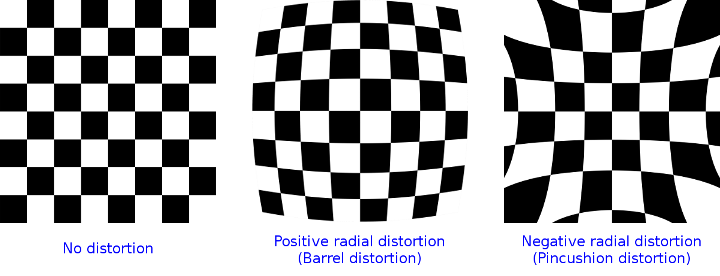
\includegraphics[height=8.5cm,width=3.5cm]{3.png}}s
            \subfigure[枕形失真]{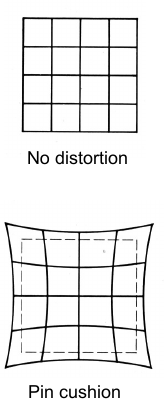
\includegraphics[height=8.5cm,width=3.5cm]{4.png}}
            \caption{径向畸变}
            \label{fig:dis1}
        \end{figure}
    \item
        由于镜头制作时感光元平面与镜头不平行,会导致切向畸变,如Fig. \ref{fig:dis2}。切向畸变一般用两个参数确定,且可以建模如下:
        \begin{equation}
            \label{eq:dis2}
            \begin{aligned}
                x_{undistorted} =& x + [ 2p_1xy + p_2(r^2+2x^2)] \\ 
                y_{undistorted} =& y + [ p_1(r^2+ 2y^2)+ 2p_2xy]
            \end{aligned}
        \end{equation}
        \begin{figure}[htbp]
            \centering
            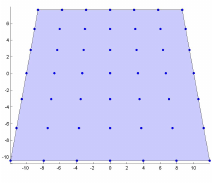
\includegraphics[height=4.5cm,width=5.5cm]{5.png}
            \caption{切向畸变}
            \label{fig:dis2}
        \end{figure}
\end{itemize}



\subsection{张氏标定}
标定单个相机是通过对应图像二维像素点与空间三维实际点,最终得到该相机的内参和畸变参数的过程。
一般的标定方法分为使用标定物和自标定两种。标定物又分为三维标定物和二维平面。

张氏标定法中,标定物是一个二维棋盘平面,并假定该平面在世界系中的$Z$轴坐标均为0。
通过不同的角度拍摄标定物,得到一组图像。针对每幅图像进行角点检测,通过对应图像中的角点与3维空间角点坐标,构建相应的坐标转换公式。
一般选取10张图片来求解。
完整的标定过程大致如下:
\subsection{获取标定图像}
打印一张棋盘格并贴在平面上作为标定物。通过变换拍摄视角或标定物方向,拍摄一组照片。
\subsubsection{提取成像平面角点}
我们选择棋盘交叉点即角点作为标定点。通过角点检测可以找到每幅图中各个角点的像素位置。
\subsubsection{提取亚像素角点信息}
\begin{figure}[htbp]
    \centering
    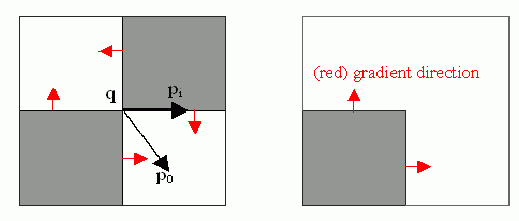
\includegraphics[height=4.5cm,width=9.5cm]{cornersubpix.png}
    \caption{亚像素优化}
\end{figure}
对于一角点$q$,在其邻域区间内取任一点$p$,向量$\overrightarrow {qp} $一定与当前点$q$所在邻域内$p$点的灰度梯度方向的转置正交,即$\overrightarrow {qp} {\rm{ }} \cdot {\rm{ }}D{I_p}^T = 0$,于是有待最小化的误差式:
\begin{equation}
    \epsilon _i = {DI_{p_i}}^T \cdot (q - p_i)
\end{equation}
其中${DI_p}^T$是p点的梯度方向转置。
\subsubsection{标定计算过程}
初始化每幅图像的角点的三维空间坐标
在得到多组点对$(x_{i,j},X_{i,j})$的情况下,我们希望求解出相机内参和畸变参数。

\begin{itemize}
    \item 首先针对每幅图像的点对,估计成像平面与棋盘平面的单应矩阵$H$
     $$
      H =\left[\begin{array}{ccc}h_1&h_2&h_3 \end{array}\right]= \lambda K \left[\begin{array}{ccc}r_1&r_2&t \end{array}\right]
     $$
    \item 因为$r_1$与$r_2$正交,因此有
    $$
    \left\{
    \begin{array}{l}h_1^TK^{-T}K^{-1}h_2 = 0 \\ h_1^TK^{-T}K^{-1}h_1 = h_2^TK^{-T}K^{-1}h_2 = 1\end{array}
    \right. 
    $$
    令$B=K^{-T}K^{-1}$,$b=[B_{11},B_{12},B_{22},B_{13},B_{23},B_{33}]$
    $$
    \Rightarrow 
    \left\{ \begin{array}{l}v_{12}^Tb = 0 \\ v_{11}^Tb = v_{22}^Tb \end{array}\right.
    $$
    \item 通过扩展每幅图像的$v$,得到$V$,并且有$Vb=0$成立,$b$是$V^T V$的特征向量。
    \item 根据$b$得到$B$,并进行cholesky分解得到$K$矩阵
    \item 在求解出$H,K$的情况下,利用旋转矩阵的正交性质求解外参
    $$
    \left\{
    \begin{aligned}
        r_1&=\lambda A^{-1} h_1 \\
        r_2& = \lambda A^{-1} h_2 \\
        r_3 &=r_1*×r_2 \\
        t&=\frac{1}{\lambda} K^{-1} h_2 \\
        \lambda &= \|K^{-1}h_1\|
    \end{aligned}
    \right.
    $$
    \item 根据通过闭合形式求解到的内、外参数,使用最小二乘,估计畸变参数
    \item 构造极大似然估计函数,使用LM算法进行所有参数的迭代优化
\end{itemize}
\subsubsection{评价}
根据计算出的内参、外参以及畸变参数,计算三维角点转换后的像素坐标与之前检测出的坐标差距,衡量参数求解的精度水平。
\subsubsection{标定效果}
根据计算出的畸变参数,将整幅图像进行矫正恢复。

该过程是通过公式(\ref{eq:dis1})和(\ref{eq:dis2}),形成像素坐标的映射关系,再根据灰度不变性形成新的图像。


\section{实验结果}
实验数据总共包含两组,且每组数据充分,因此针对单个相机都进行了多组数据的交叉验证。
也就是使用部分图片用来做参数的求解,将求解出来的参数应用到剩余图像上来观察效果,并对求出的多组参数进行统计,将求解的参数分别进行角点重投影,计算像素坐标的误差。

\begin{table}[htbp]
\centering
\caption{内参矩阵结果对比}
	\begin{tabular}{|c|c|c|c|}
	\hline 
	相机 & 1 & 2 & 3 \\ 
	\hline 
	Mode1 & • & • & • \\ 
	\hline 
	Mode2 & • & • & • \\ 
	\hline 
	\end{tabular} 
\end{table}

\begin{table}[htbp]
    \centering
    \caption{畸变参数结果对比}
        \begin{tabular}{|c|c|c|c|}
        \hline 
        相机 & 1 & 2 & 3 \\ 
        \hline 
        Mode1 & • & • & • \\ 
        \hline 
        Mode2 & • & • & • \\ 
        \hline 
        \end{tabular} 
    \end{table}

\section{结果评估与误差源分析}
将求解的参数应用到图像上,观察畸变参数的准确性

\begin{enumerate}[(1)]
    \item 图像数量
    
    为了获得稳定的数值结果,通常采集的图片数量会远远超过次数。
    如果采集图像不足,明显会对内部参数计算带来一定的误差,
    但采集图像过多一方面影响标定的精度,另一方面也会造成误差累积,增加错误概率。因此合适图像数量必须加以考虑。
    \item 标定板制作误差
    
    制作标定板时,往往都假设打印的黑白棋盘格是等边长的[7]。但是由于普通打印机不够精确,造成了测量标定板的误差。
    \item 角点检测
    
    角点提取算法决定了角点的像素坐标的精度。标定的计算依赖于点对。
    \item 标定板所在平面与成像平面之间的夹角太小
    
    在阅读张正友论文时注意到,他使用的仿真数据(有噪声的数据)说明当两者夹角太小误差会很大。
    同时图像之间的视角也应该有较大差距。
\end{enumerate}
\end{CJK*}
\end{document}